\documentclass{beamer} % [aspectratio=169]
\usetheme{ucl}
\setbeamercolor{banner}{bg=darkred}
\setbeamersize{description width=2em}
\setbeamertemplate{navigation symbols}{\vspace{-2ex}} 

%\usepackage{fontspec}
\usepackage[utf8]{inputenc}
% \usepackage[english, greek]{babel}


\usepackage[T1]{fontenc} % Turn £ into $
\usepackage{minted}
\usemintedstyle{emacs}

\usepackage{fancyvrb}
\usepackage{xcolor}
\usepackage{url}

\usepackage{natbib}
\usepackage{bibentry}
\usepackage{url}


\usepackage{tikz}
\usetikzlibrary{positioning}


\newcommand\emc[1]{\textcolor{midred}{\textbf{#1}}}

\AtBeginSection[]{
  \begin{frame}
  \vfill
  \centering
  \begin{beamercolorbox}[sep=8pt,center,shadow=true,rounded=true]{title}
    \usebeamerfont{title}\insertsectionhead\par%
  \end{beamercolorbox}
  \vfill
  \end{frame}
}

\author{Prof.\ Mark Handley, University College London, UK\\
\vspace{3mm}\tiny{Based in part on slides from George Danezis}}
\title{Introduction to Data Structures and Algorithms.}
\subtitle{ENGF0002: Design and Professional Skills }
% \institute{}
\date{Term 1, 2018}


\begin{document}
\nobibliography*


\frame{
\titlepage
}

\section{Lists}

\begin{frame}
  \frametitle{Python Lists}
	\inputminted[
		xleftmargin=1.4em,
		%frame=lines,
		%framesep=2mm,
		%baselinestretch=1.2,
		bgcolor=stone,
		fontsize=\footnotesize,
		%linenos
	]{python}{src/interactive_lists.py}
\end{frame}

\begin{frame}
  \frametitle{List Performance}
  How do Python lists perform?
  
  \vspace{5mm}
  How are Python lists actually implemented?
\end{frame}

\begin{frame}
  \frametitle{Python Lists: append performance}
	\inputminted[
		xleftmargin=1.4em,
		%frame=lines,
		%framesep=2mm,
		%baselinestretch=1.2,
		bgcolor=stone,
		fontsize=\footnotesize,
		%linenos
	]{python}{tests/testappend.py}
        Append a number to a list 10 million times.  Print out elapsed time every 10,000 appends.
\end{frame}

\begin{frame}
  \frametitle{Python Lists: append performance}
  \centering
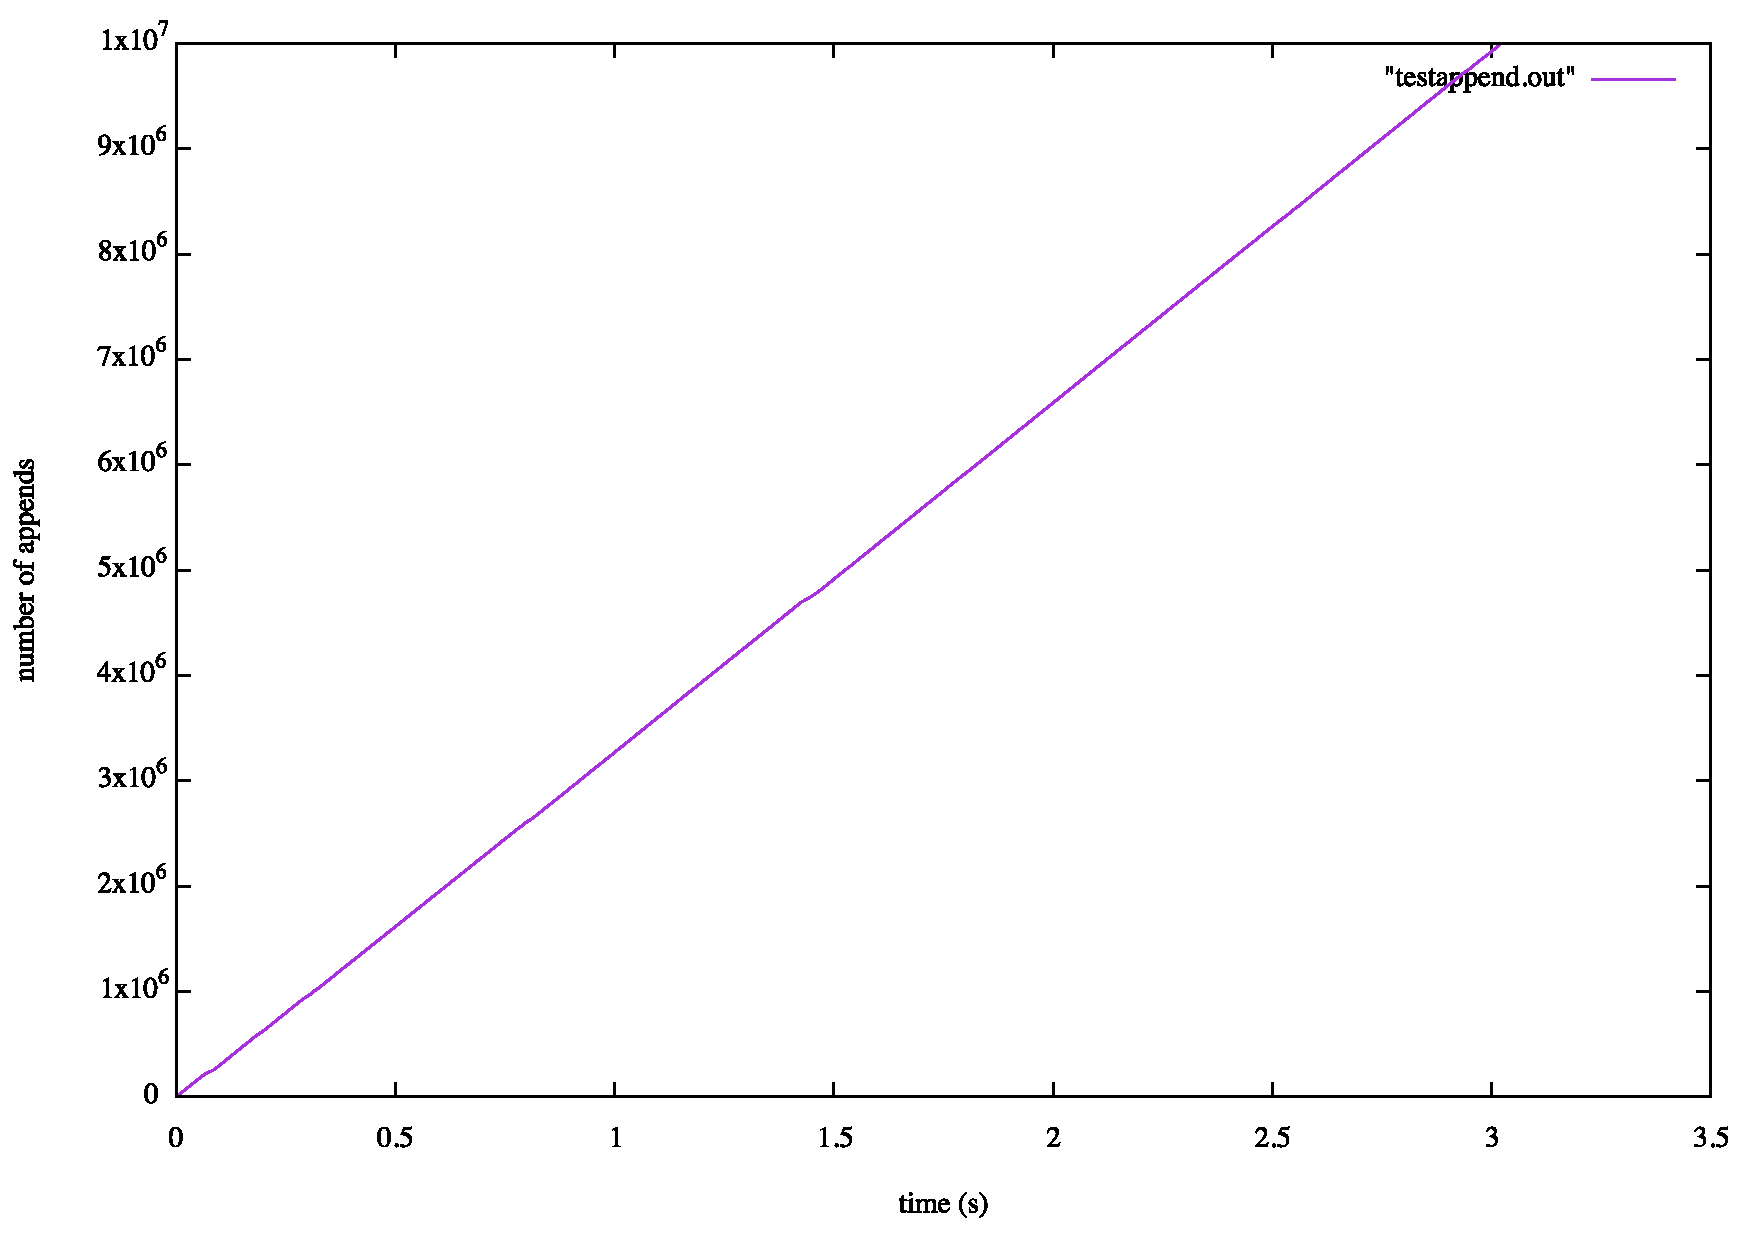
\includegraphics[height=75mm]{tests/testappend.pdf}
\end{frame}

\begin{frame}
  \frametitle{Python Lists: del performance}
	\inputminted[
		xleftmargin=1.4em,
		%frame=lines,
		%framesep=2mm,
		%baselinestretch=1.2,
		bgcolor=stone,
		fontsize=\footnotesize,
		%linenos
	]{python}{tests/testdel1.py}
        Create a 10 million item list.  Delete front item, print out elapsed time every 10,000 delettions.
\end{frame}

\begin{frame}
  \frametitle{Python Lists: del performance}
	\inputminted[
		xleftmargin=1.4em,
		%frame=lines,
		%framesep=2mm,
		%baselinestretch=1.2,
		bgcolor=stone,
		fontsize=\footnotesize,
		%linenos
	]{python}{tests/testdel4.py}
        Create a lists of increasing length.  Time how long it takes to remove 200 items.
\end{frame}

\begin{frame}
  \frametitle{Python Lists: deletion performance}
  \centering
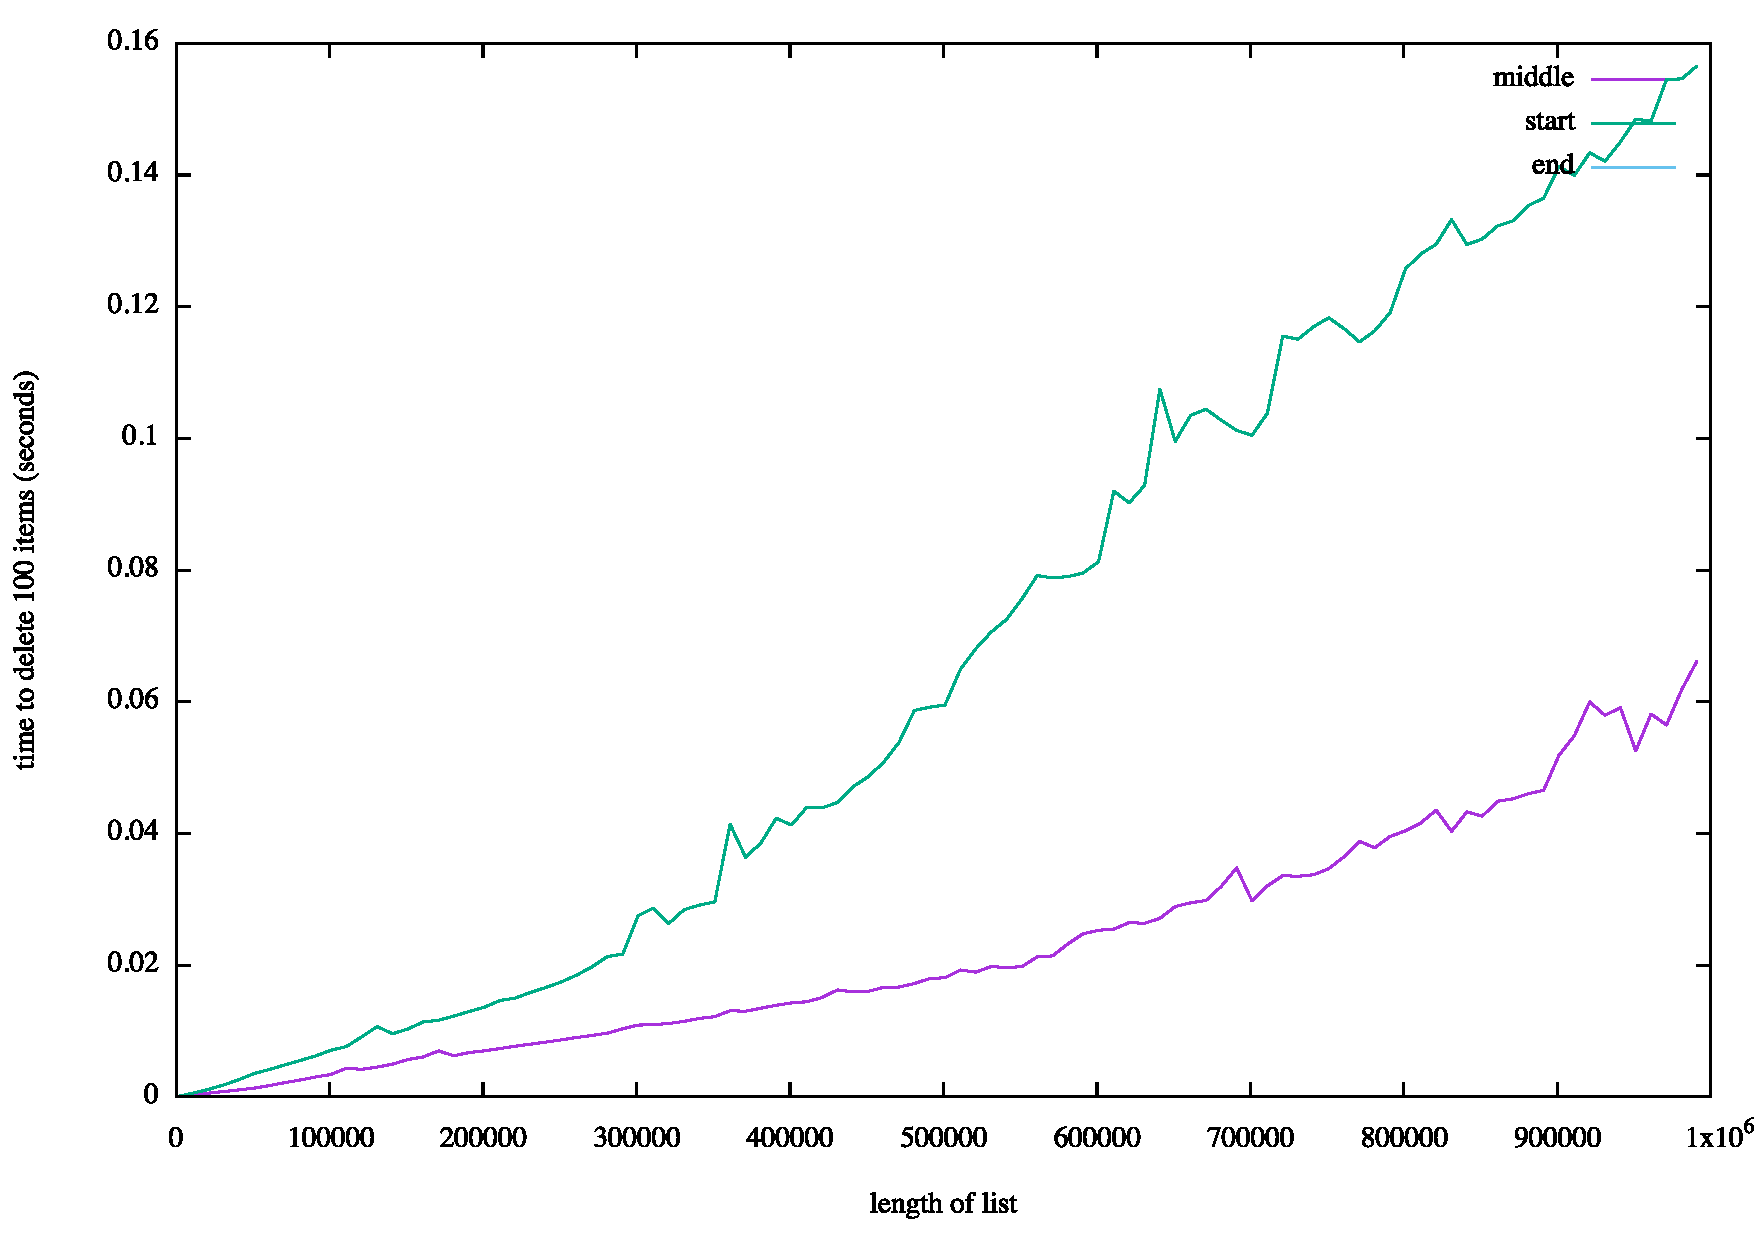
\includegraphics[height=75mm]{tests/testdel4-5-6.pdf}
\end{frame}

\begin{frame}
  \frametitle{Python Lists: deletion performance, logscale}
  \centering
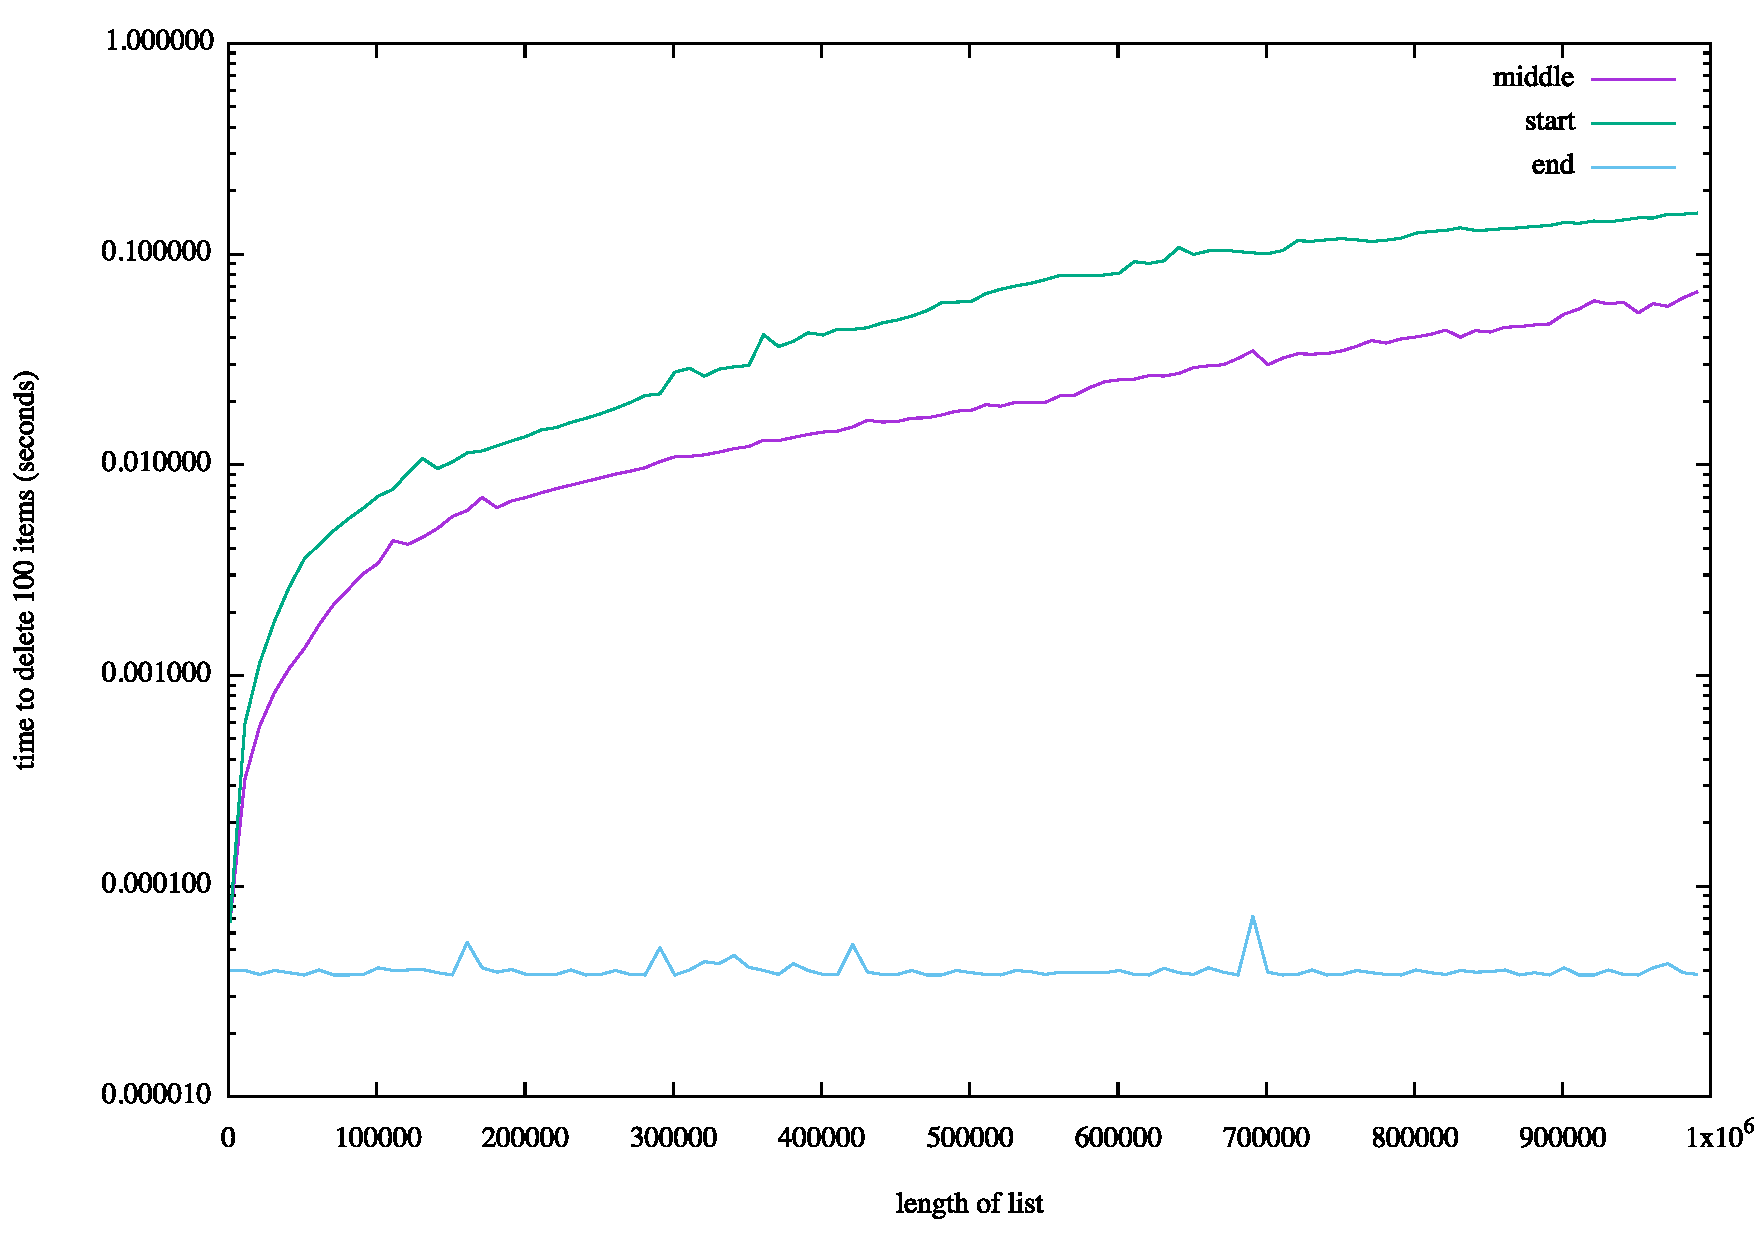
\includegraphics[height=75mm]{tests/testdel4-5-6-log.pdf}
\end{frame}

\begin{frame}
  \frametitle{Python Lists: performance accessing items}
	\inputminted[
		xleftmargin=1.4em,
		%frame=lines,
		%framesep=2mm,
		%baselinestretch=1.2,
		bgcolor=stone,
		fontsize=\footnotesize,
		%linenos
	]{python}{tests/testaccess.py}
        Create a lists of increasing length.  Time how long it takes to access 1000 items.
\end{frame}

\begin{frame}
  \frametitle{Python Lists: performance accessing items}
  \centering
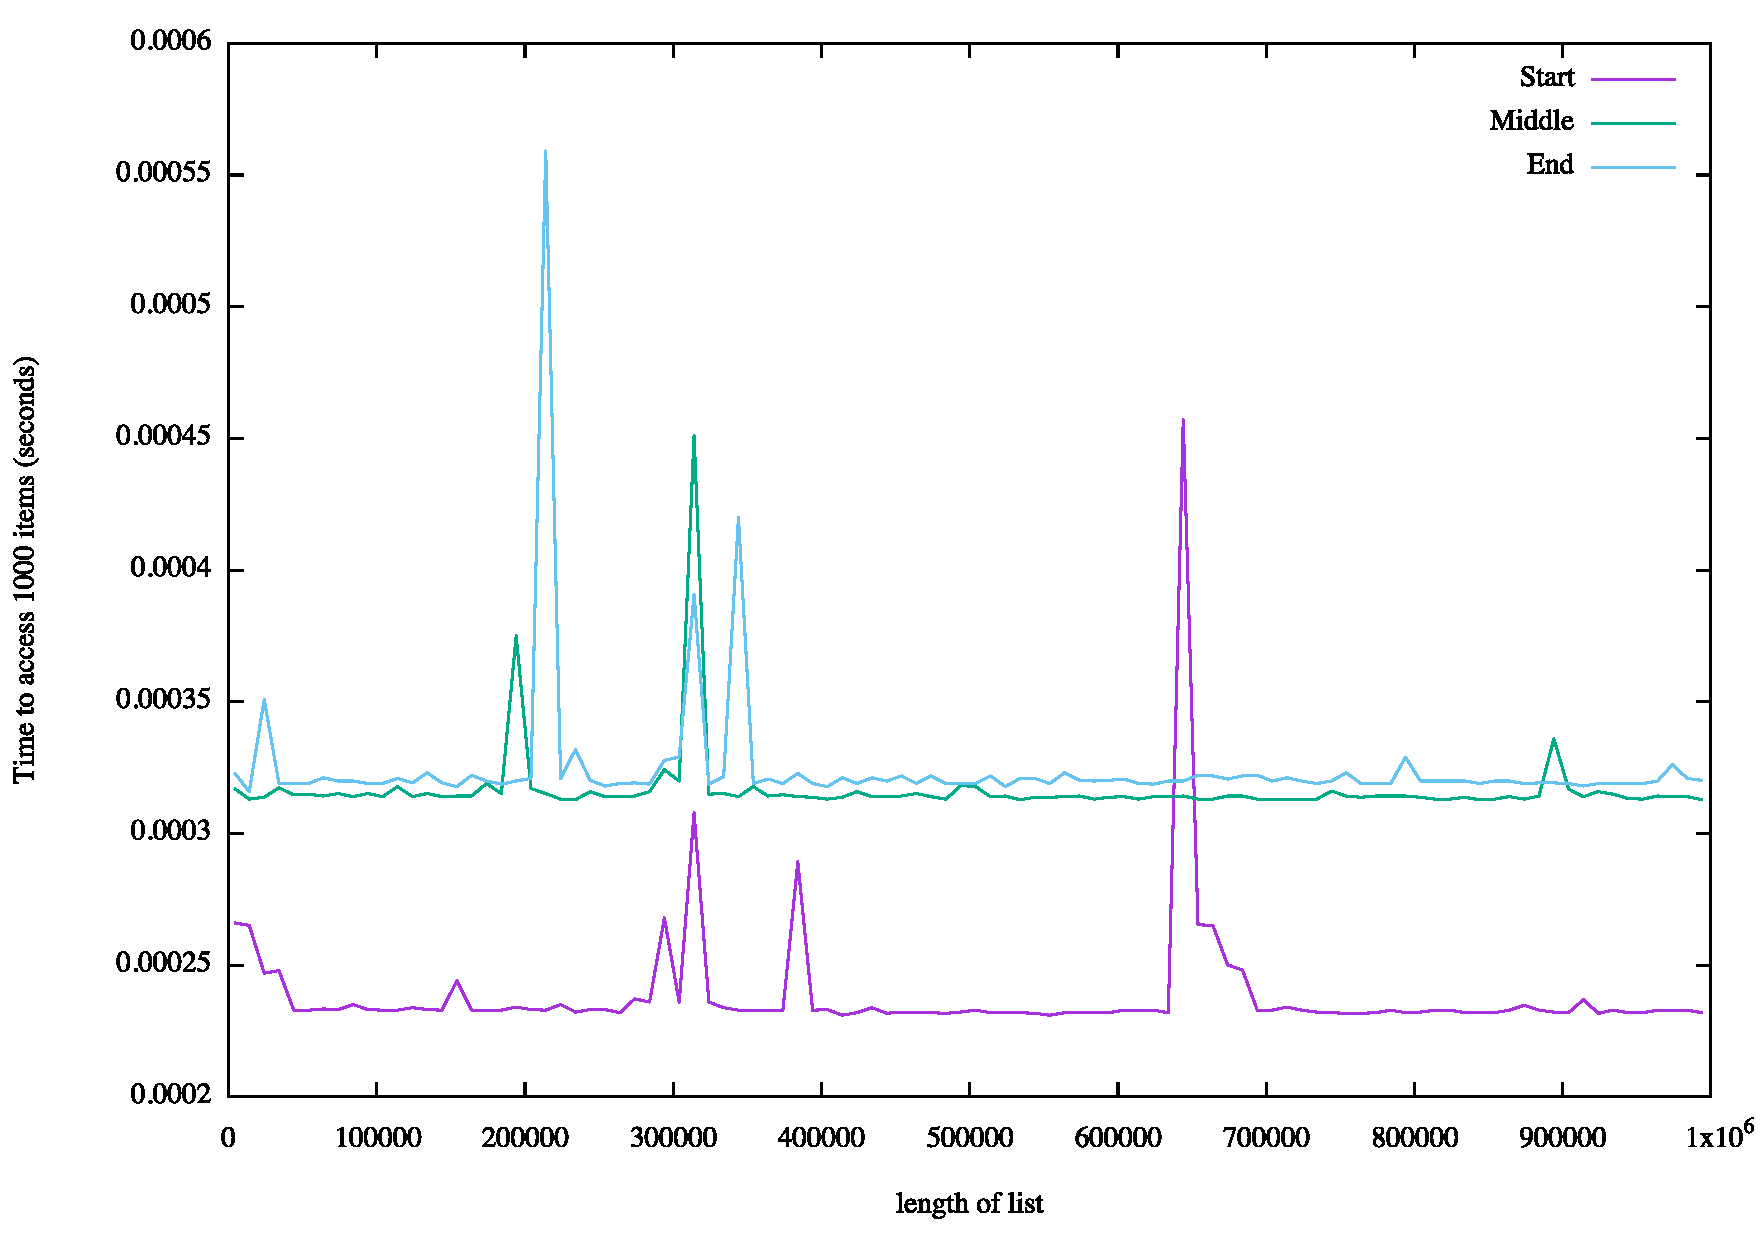
\includegraphics[height=75mm]{tests/testaccess.pdf}
\end{frame}

\begin{frame}
  \frametitle{Profiling and Visualization}
  A profiler is software that analyzes what other software is doing.

  \vspace{2mm}
  Many different profilers exist; can profile different resources and at different levels.

  \vspace{2mm}
  Can we find out for sure where python is spending its time?
  \begin{itemize}
  \item A python profiler won't help - will tell us it's spending its time in pop()
  \item Need to profile the python interpreter itself.
  \end{itemize}
\end{frame}

\section{Visualization}

\begin{frame}
  \frametitle{Profiling: dtrace}
  Advanced topic, you don't need to know this yet.  Rough summary:

  \begin{itemize}
  \item I used dtrace to connect to the running python interpreter process.
  \item 1000 times per second, interrupted it, and logged what function was being called (known as a stack trace)
  \item Dumped the stats as a profile trace.
  \item Ran some fancy perl scripts to visualize the data.
  \end{itemize}
\end{frame}
    
\begin{frame}
  \frametitle{Flame graph of deletion from end}
  \centering
  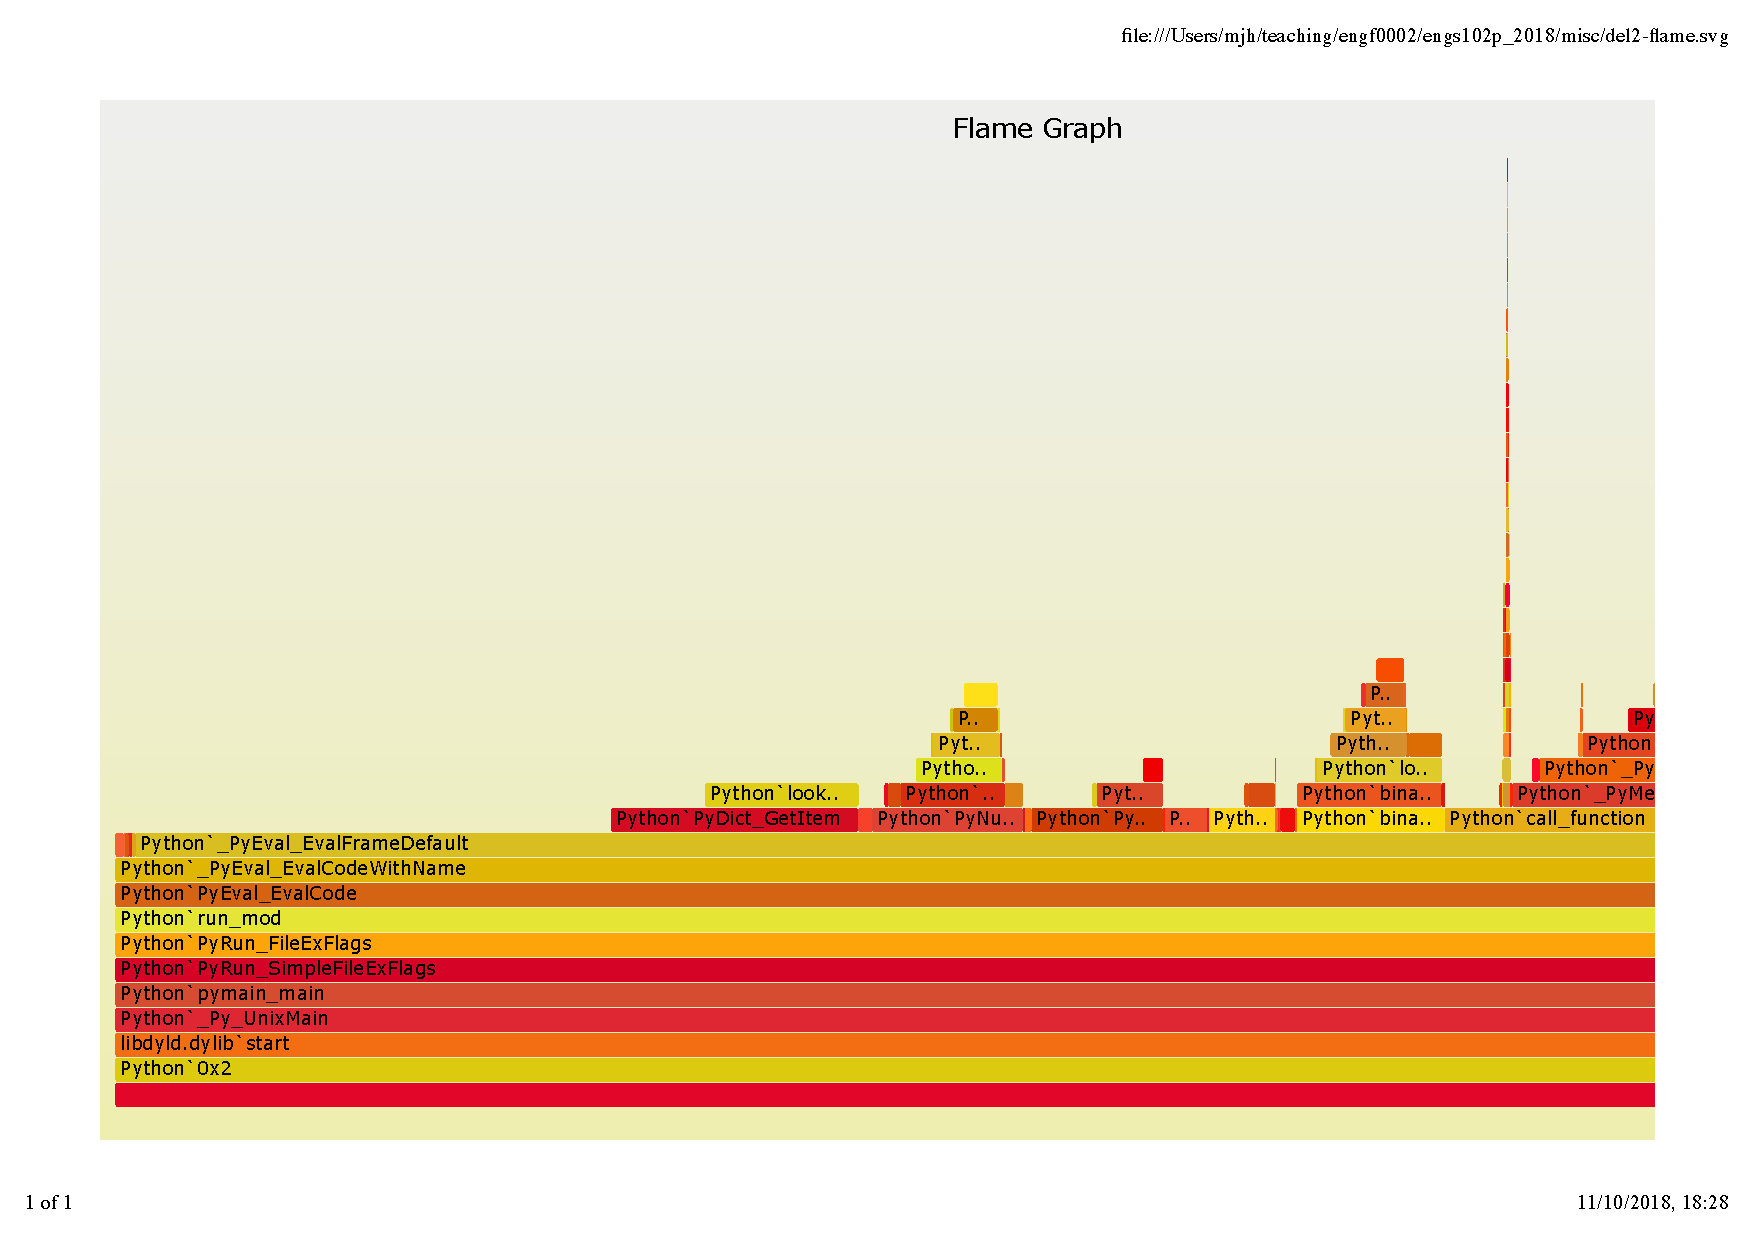
\includegraphics[height=75mm]{assets/del2-flame.pdf}
\end{frame}
  
\begin{frame}
  \frametitle{Flame graph of access from middle}
  \centering
  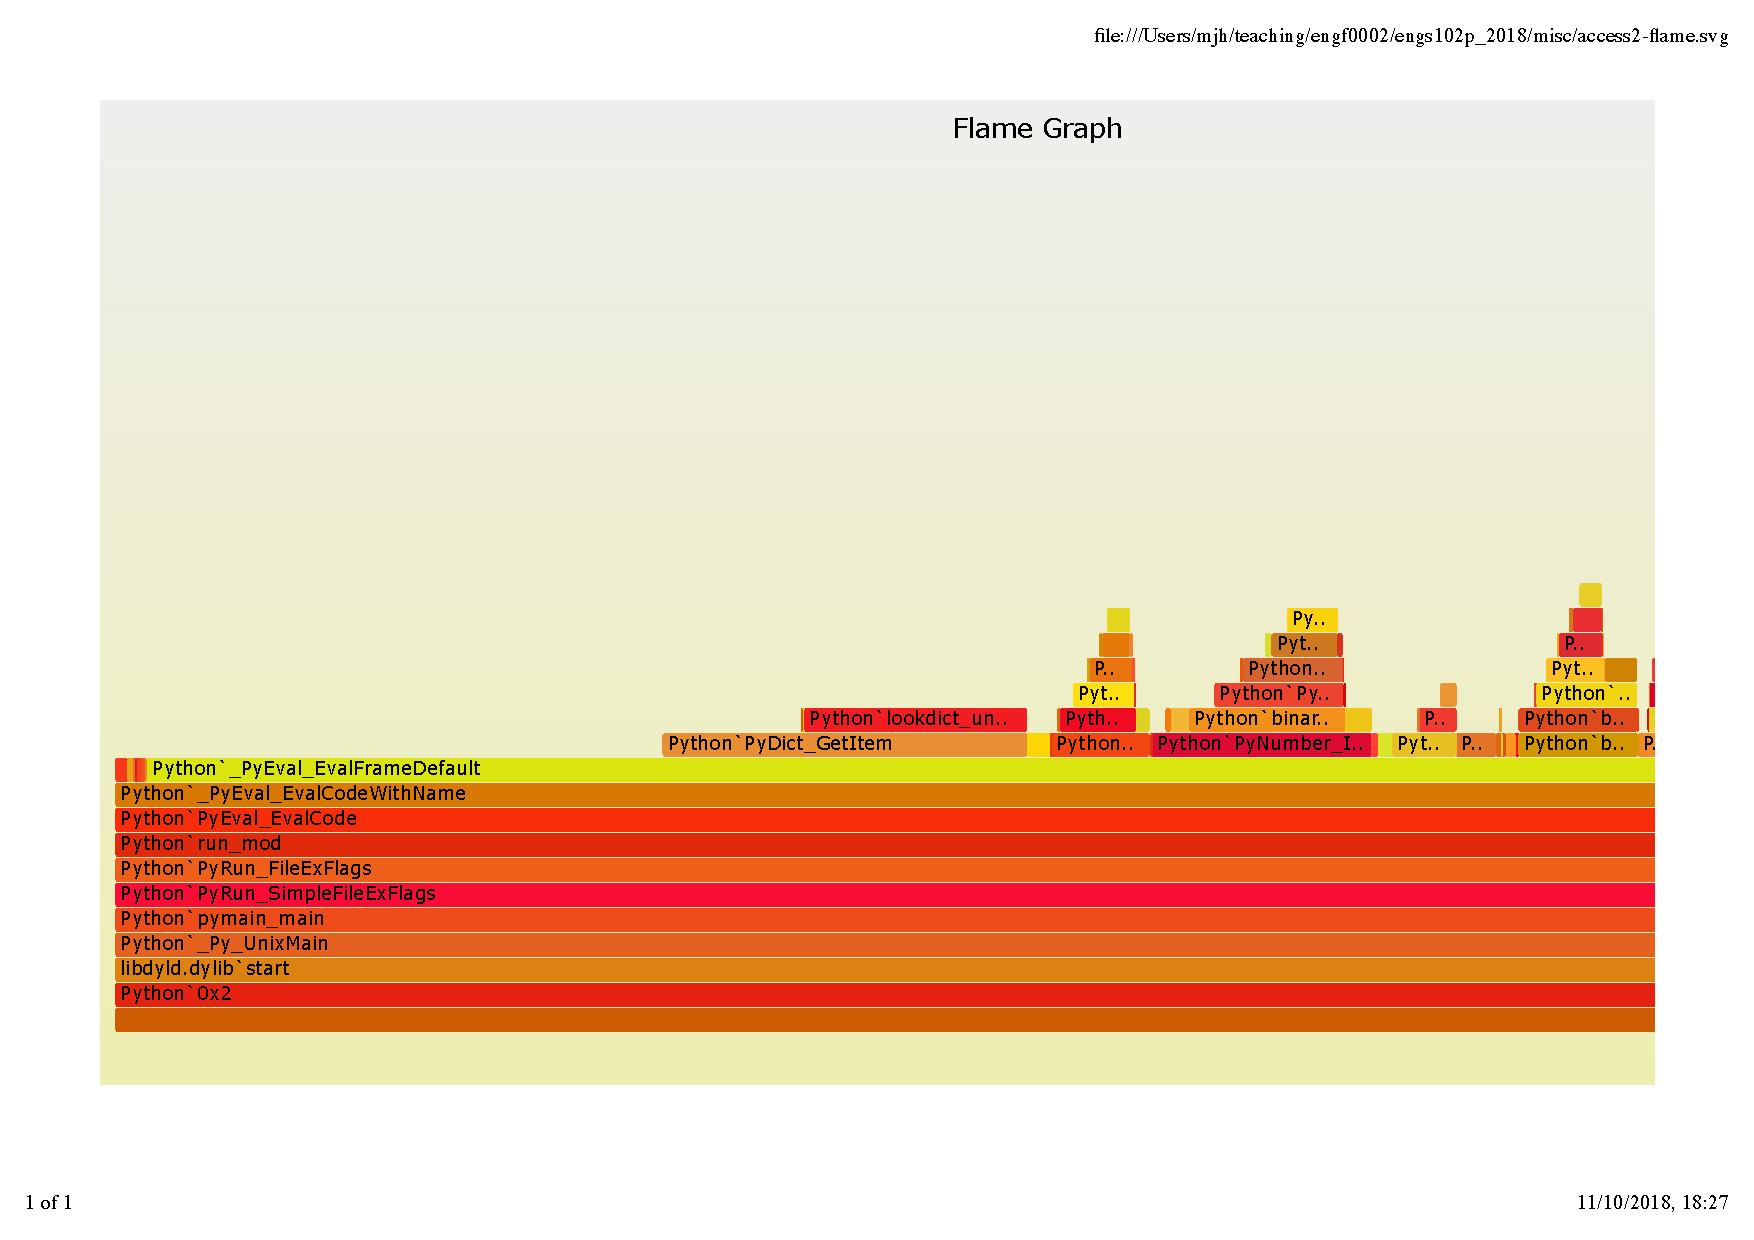
\includegraphics[height=75mm]{assets/access2-flame.pdf}
\end{frame}
  
\begin{frame}
  \frametitle{Flame graph of deletion from beginning}
  \centering
  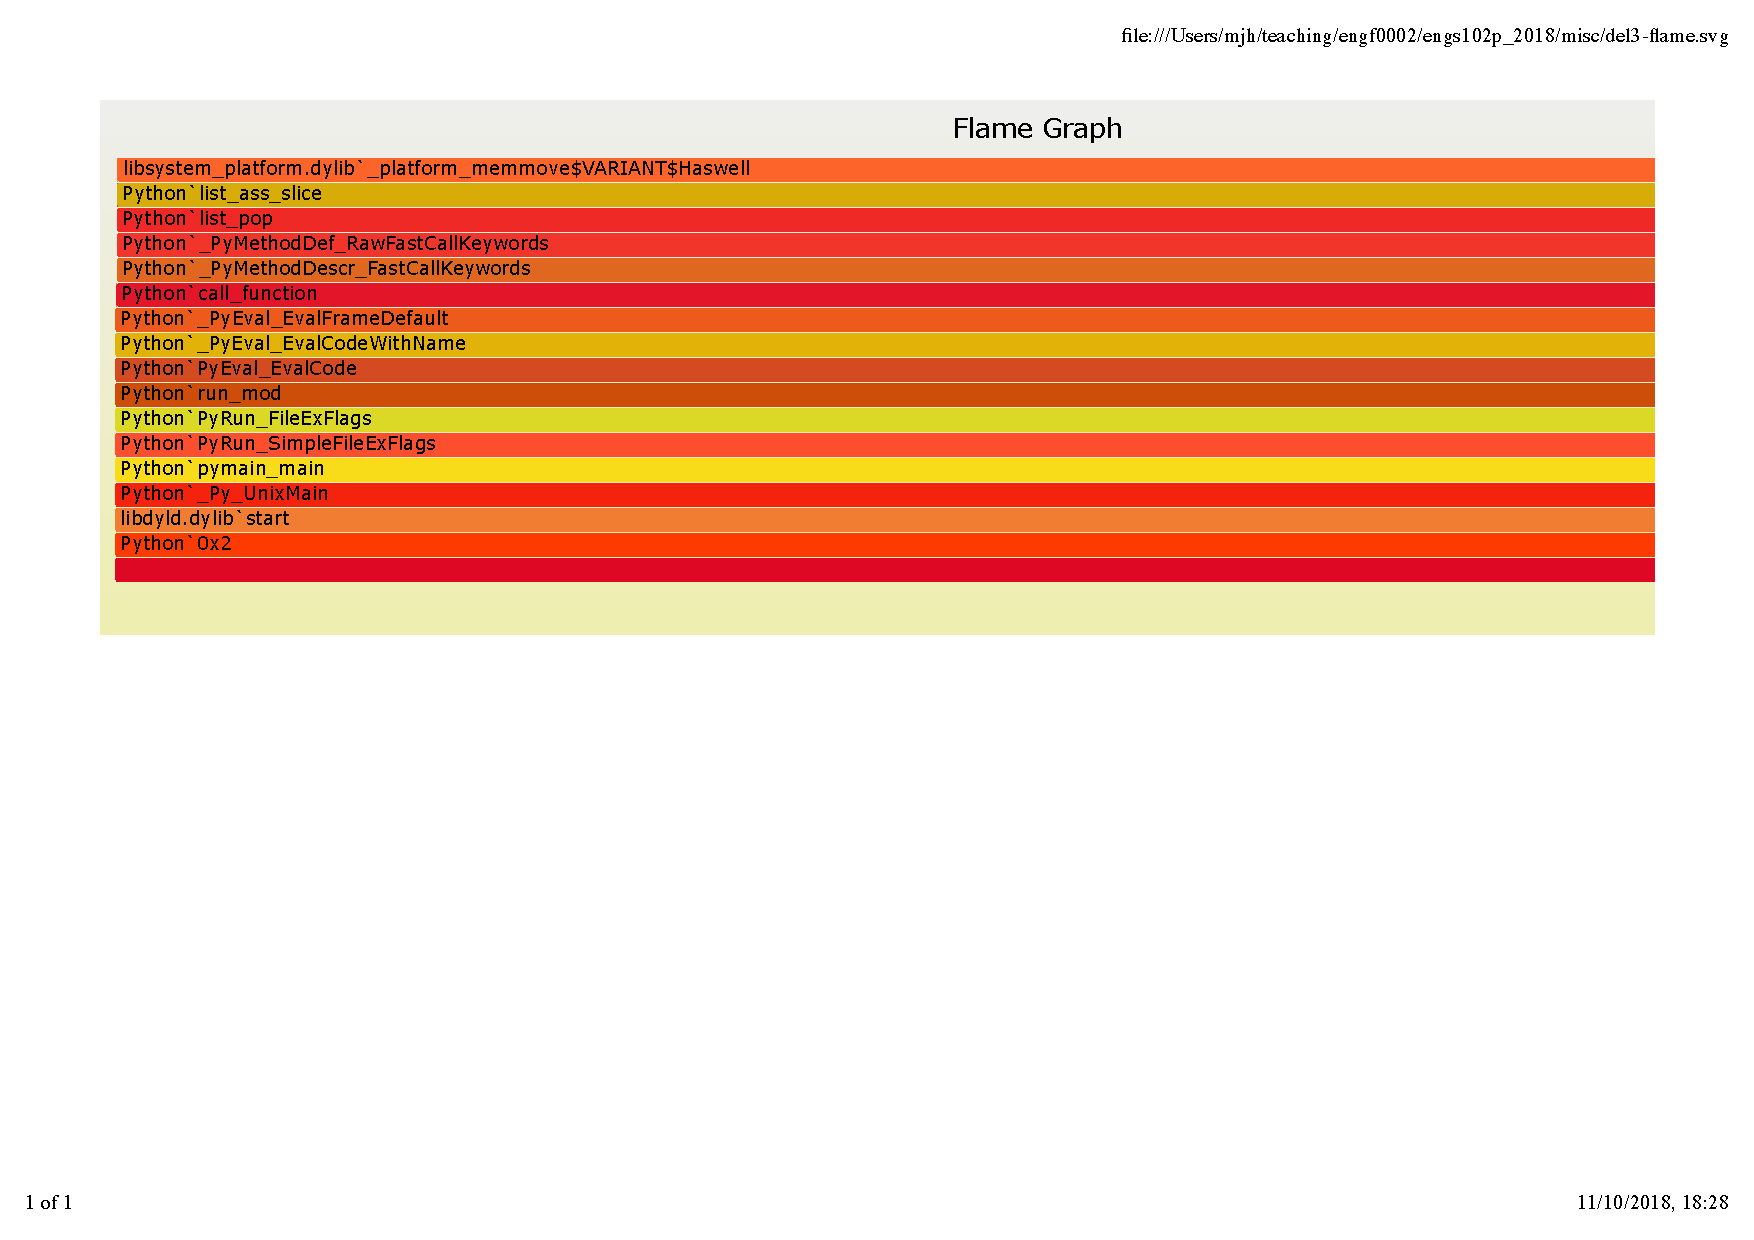
\includegraphics[height=75mm]{assets/del3-flame.pdf}
\end{frame}

\begin{frame}
  \frametitle{The Importance of Good Visualization}
  \centering
  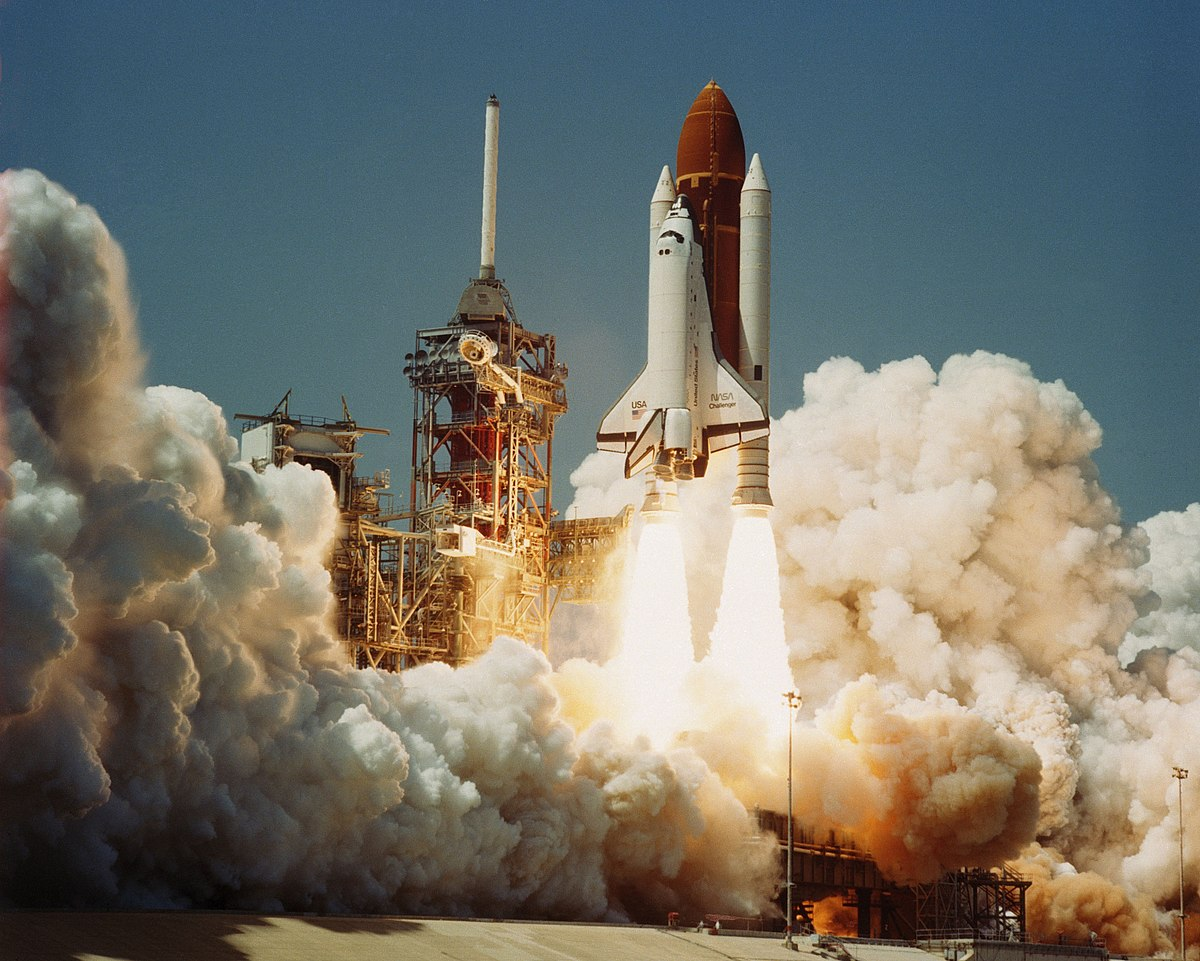
\includegraphics[height=75mm]{assets/challenger.jpg}
\end{frame}

\begin{frame}
  \frametitle{Graph from Thiokol's presentation to NASA}
  \centering
  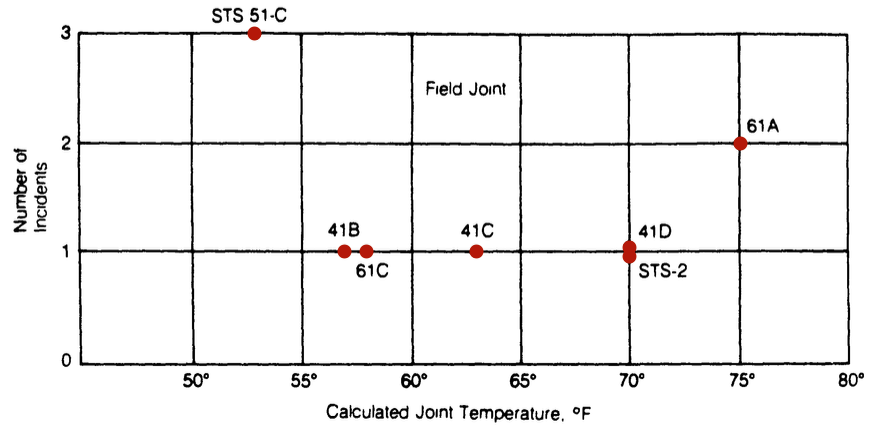
\includegraphics[width=120mm]{assets/thiokol-challenger-graph.png}
\end{frame}

\begin{frame}
  \frametitle{Edward Tufte's version of the same data}
  \centering
  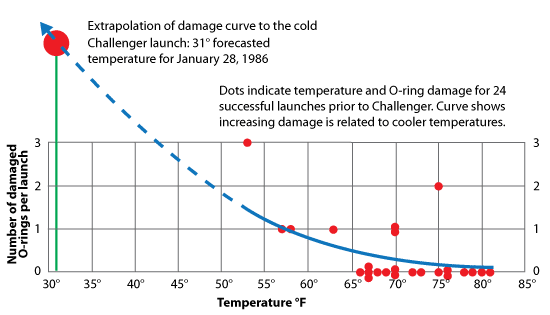
\includegraphics[width=120mm]{assets/tufte-challenger-graph.png}
\end{frame}

\section{Algorithms \& computational complexity}

\begin{frame}
  \frametitle{The Bookshop Problem}
  \centering
  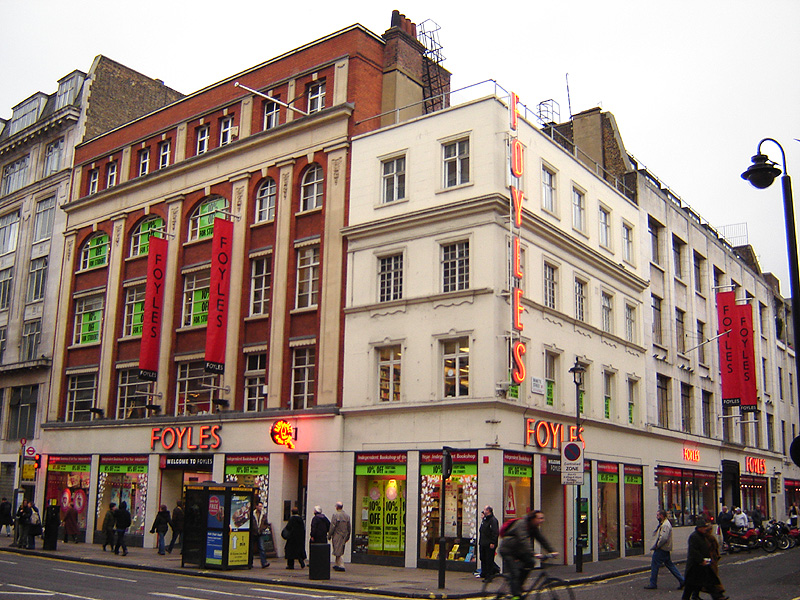
\includegraphics[width=110mm]{assets/foyles.jpg}
\end{frame}

\begin{frame}
  \frametitle{The Bookshop Problem: Solution}
  \centering
  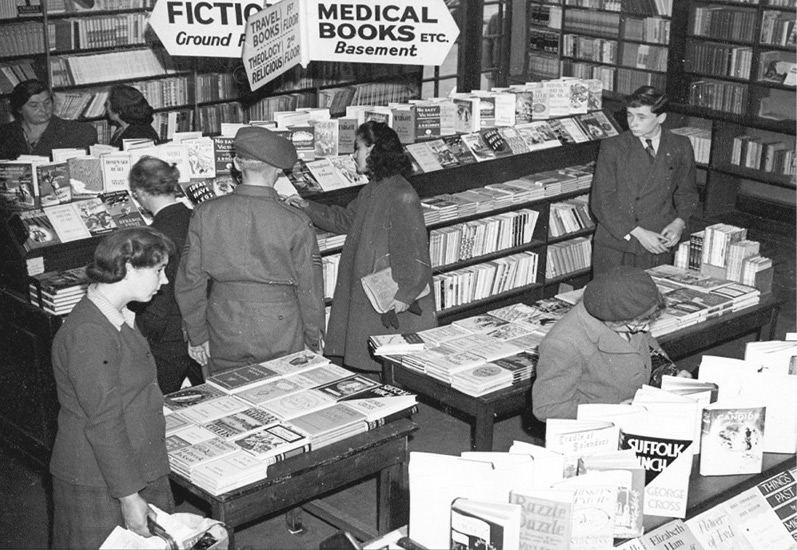
\includegraphics[height=70mm]{assets/foyles2.jpg}
  
  Best known algorithm: find Christina Foyle and ask her.
\end{frame}

\begin{frame}
  \frametitle{Is a value stored in a list?}

Basically the same problem as Foyles bookshop.

\vspace{3mm}
We wish to define an algorithm \texttt{is\_in} to test whether a list contains a target value.
\begin{itemize}
\item Return \texttt{True} if it is, and \texttt{False} otherwise.
\end{itemize}

\vspace{3mm}
Some \emc{simple tests} for \texttt{is\_in} would be:
	\inputminted[
		firstline=1,
		lastline=3,
		xleftmargin=1.4em,
		%frame=lines,
		%framesep=2mm,
		%baselinestretch=1.2,
		bgcolor=stone,
		fontsize=\footnotesize,
		%linenos
	]{python}{src/isin.py}

\end{frame}

\begin{frame}
\frametitle{Sequential search.}

	\inputminted[
		firstline=5,
		lastline=9,
		xleftmargin=1.4em,
		%frame=lines,
		%framesep=2mm,
		%baselinestretch=1.2,
		bgcolor=stone,
		fontsize=\footnotesize,
		%linenos
	]{python}{src/isin.py}

\begin{itemize}
	\item We construct a function that takes as parameters a list (\texttt{lst}) and target value (\texttt{target}).
	\item It uses a \texttt{for} loop to sequentially go through all the values of \texttt{lst}.
	\item Within the loop each value is tested. If they match return \texttt{True}.
	\item If the loop completes, it returns \texttt{False}.
\end{itemize}

\end{frame}

\begin{frame}
\frametitle{How efficient is the \texttt{is\_in} algorithm?}

Assume the list has $n$ elements:
\begin{itemize}
\item The algorithm will iterate over $n$ elements if it returns \texttt{False}.
\item If the target value is at a random position it will iterate on average over $\frac{1}{2} n$ elements.
\end{itemize}

\vspace{5mm}
The number of specific steps executed, as a function of the size of its inputs is a key measure of the \emc{time complexity} of an algorithm.

\vspace{5mm}
However, we often only care about time complexity increases \emc{within a constant factor} and for \emc{large enough parameter sizes}.

\end{frame}

\begin{frame}
\frametitle{The $\mathcal{O}$ (Big Oh) notation.}

Lets call the average number of steps an algorithm takes $f(n)$. We define as the \emc{order of} relation between functions.

\vspace{3mm}
We say that $f(n) = \mathcal{O}(g(n))$ as $n \rightarrow \infty$ if

\[ \exists n_0, c > 0. \quad |f(n)| \leq c \cdot |g(n)| \quad \text{ for } n \geq n_0. \]

\begin{itemize}
\item In words, there exists a value $n_0$ after which the function $f(n)$ is always smaller than $g(x)$ up to a constant $c$.
\item Note that the notation \emc{hides lower order terms and constant}, \\ eg. $3n^2 + 10n + 5 = \mathcal{O}(n^2)$.
\end{itemize}

\begin{block}{}
Sequential search has time complexity in the order of $\mathcal{O}(n).$
\end{block}

\end{frame}


\begin{frame}
\frametitle{Can we search a sequence in fewer steps?}

An arbitrary sequence cannot be searched in time less than $\mathcal{O}(n)$.

\vspace{3mm}
However, we can \emc{pre-compute an index} on the sequence:
\begin{itemize}
	\item An index is \emc{a sorted view} of a sequence that allows fast \emc{is\_in} operations.
\end{itemize}

\end{frame}


\begin{frame}
  \frametitle{Binary search algorithm}
  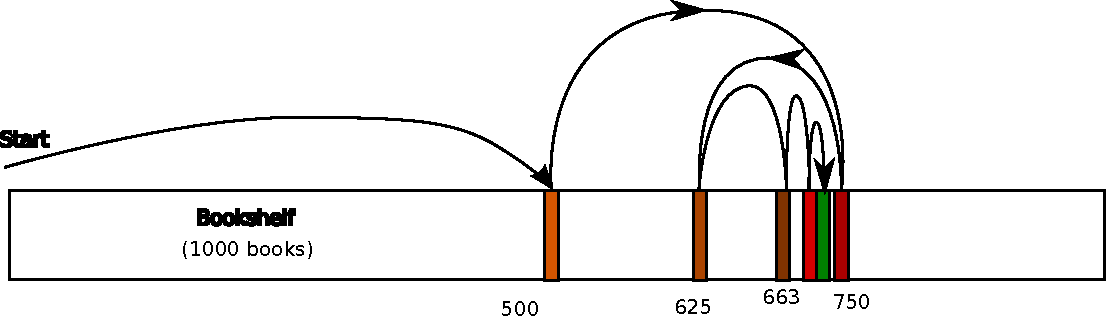
\includegraphics[width=120mm]{assets/bookshelf.pdf}
\end{frame}

\begin{frame}
  \frametitle{How long does the search take?}
  \begin{center}
\begin{tabular}{ccc}
Step & Books Eliminated & Books Remaining\\
\hline
1 & 500 & 500\\
2 & 750 & 250\\
3 & 875 & 125\\
4 & 938 & 62\\
5 & 969 & 31\\
6 & 984 & 16\\
7 & 992 & 8\\
8 & 996 & 4\\
9 & 998 & 2\\
10 & 999 & 1
\end{tabular}
\end{center}
\end{frame}

\begin{frame}
  \frametitle{The story of Sissa ben Dahir and the rice}
  \centering
  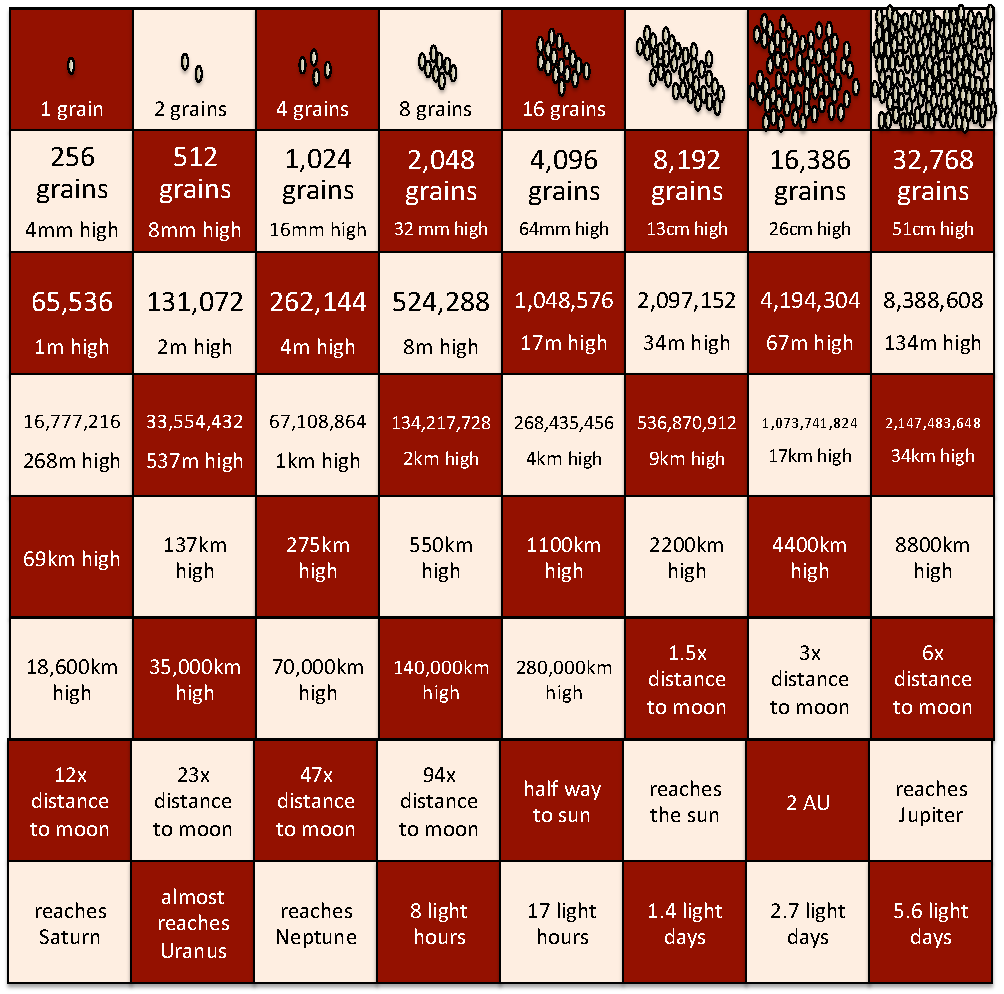
\includegraphics[height=75mm]{assets/chessboard.pdf}
\end{frame}

\begin{frame}
\frametitle{Binary search algorithm} 

\begin{itemize}
\item Define two variables \texttt{start} and \texttt{end}, initialized with the indexes of the first element and one past the last element
\item Pick the middle element of the range.
  \begin{itemize}
  \item if it is larger than the value sought, target is in lower half of the range.  {\tt end} takes the value of \texttt{middle}.
  \item otherwise target is in upper half of range.  \texttt{start} takes the value of \texttt{middle}
  \end{itemize}
\item Repeat until the range is of size one.
\item If the element at the start of the range is the target value, return \texttt{True}. 
\item Otherwise, return \texttt{False}.
\end{itemize}

\end{frame}

\begin{frame}
\frametitle{The code for binary search.}

        \inputminted[
                firstline=14,
                lastline=26,
                xleftmargin=1.4em,
                %frame=lines,
                %framesep=2mm,
                %baselinestretch=1.2,                                           
                bgcolor=stone,   
                fontsize=\footnotesize,
                %linenos
        ]{python}{src/binarysearch.py}

\end{frame}

\begin{frame}
\frametitle{Binary search has $\mathcal{O}(\log n)$ time complexity.}

\textbf{Proof.} Consider the size of the range $n = end - start$.  $n = n_0$ at step 0. At each step the size of the range is a fraction $0 < \alpha < 1$ of its previous size, namely $n_i = \alpha \cdot n_{i-1}$.  As we do integer division by 2, $\alpha \approx 0.5$
\begin{align}
  n_i &= \alpha \cdot n_{i-1} \\
  \Leftrightarrow n_i &= \alpha^i \cdot n_{0}
\end{align}
After how many steps $i$ will $n_i$ become $1$, and the algorithm end?
\begin{align}
  \alpha^i \cdot n_{0} &= 1 \\
  \Leftrightarrow \log (\alpha^i \cdot n_{0}) &= 0 \\
\Leftrightarrow i \log \alpha + \log n_{0} &= 0 \\
\Leftrightarrow i &= \left( - \frac{1}{\log \alpha} \right) \cdot \log n = \mathcal{O}(\log n).
\end{align}

\end{frame}


\begin{frame}
\frametitle{The intimate link between data structures and algorithms.}

Sequential search works on any sequence, but takes time $\mathcal{O}(n)$.

\vspace{5mm}
Binary search takes time $\mathcal{O}(\log n)$, but requires a sorted sequence. The data structure (sorted sequence) and the algorithm (binary search) work together and depend on each other.

\vspace{5mm}
\begin{block}{Is $\mathcal{O}(\log n)$ really much better than $\mathcal{O}(n)$?}
Remember $\mathcal{O}(\log n)$ is proportional to the number of binary digits in $n$ (up to a constant). So if $n=1000000$ then sequential search will take about a million steps, while binary search will take about 20. That is a big difference, and it grows as $n$ grows.
\end{block}

\end{frame}


\begin{frame}
\frametitle{Functions \& Recursion.}

A function is called \emc{recursive}, or \emc{using recursion}, if it is \emc{calling itself}!
\begin{itemize}
	\item A way of expressing a computation, possibly more naturally.
	\item Anything that can be done with recursion can be done with loops, and vice versa.
	\item Only a limited \emc{resursive depth} is allowed.
\end{itemize}

\begin{block}{What is recursion good for?}
A number of problems are naturally expressed by dividing them into \emc{sub-problems of the same form} as the initial problem. This algorithmic strategy is called \emc{divide-and-conquer} and recursion is well suited to expressing a solution.
\end{block}

\end{frame}

\begin{frame}
\frametitle{The recursive variant of binary search.}

	\inputminted[
		firstline=10,
		lastline=20,
		xleftmargin=1.4em,
		frame=lines,
		framesep=2mm,
		%baselinestretch=1.2,
		% bgcolor=lightgray,
		fontsize=\footnotesize,
		linenos
	]{python}{src/binarysearch_recurse.py}

\begin{itemize}
	\item Recursion at line 18 and 20.
	\item Other tricks: default parameters (line 10) and conditional expression (line 11).
\end{itemize}

\end{frame}

\bibliographystyle{alpha}
\nobibliography{references}

\end{document}
